\section{Texto e Código} %------------------------------------------------------
\label{sec:textoCodigo}

\begin{margintable}\vspace{.8in}\footnotesize
  \caption{Sumário da \textsc{part III}}
  \medskip
  \begin{tabularx}{\marginparwidth}{|X}
    \textbf{\sffamily \textcolor{azulUFRB}{Seção}~\ref{sec:textoCodigo}}.    {\sffamily Texto e Código} \\
    \textbf{\sffamily \textcolor{azulUFRB}{Seção}~\ref{sec:fontes}}.    {\sffamily Algo sobre Fontes} \\
  \end{tabularx}
\end{margintable}

A escrita do código em \LaTeX\ possui algumas peculiaridades.
Muitas delas, dependem de subjetividade e, portanto, fica à critério de cada um.
Vou falar apenas a minha experiência.

Quando iniciei no \LaTeX\ fazia códigos na mesma linha, aglutinando comandos.
Não me preocupava se num futuro eu teria dificuldade em entender o que escrevi, 
nem do trabalho que é encontrar um erro num código bagunçado!
Existem boas práticas e, desde cedo, aconselho vocês seguirem.\nota{
  Complementando essa ideia de \textsf{boas práticas} na escrita do código, o 
  texto 
  \hrefA
  {
    https://ctan.dcc.uchile.cl/info/l2tabu/english/l2tabuen.pdf
  }
  {
    \itshape An essential guide to \hologo{LaTeX2e} usage,
  }
  traz uma boa noção de comandos e pacotes obsoletos.
  É uma boa prática, sempre que possível, usar comandos mais novos e que, muitas 
  vezes, foram criados para resolver problemas de anteriores!
}

Na realidade, já estamos fazendo isso!
De fato, definimos uma estrutura de diretórios e organização dos arquivos 
\texttt{.tex}; indicamos como nomear arquivos; usamos comentários para separar 
partes do código; etc. 
Mas, a escrita, em si, deve comtemplar alguns aspectos também!
Ao meu ver, pense que todo o seu texto seja um código!
Uma boa prática, então, é manter cada linha de seu texto com, no máximo, 80 
caracteres.
Além disso, eu costumo colocar cada parágrafo em uma linha de código.
Isso é possível, pois o \LaTeX\ não considera mais de um espaçamento entre 
palavras!
Um novo parágrafo só é formado de você deixar uma linha em branco entre ele e o
anterior.

Por exemplo:\mn{
  Vejam a forma como colocamos aspas na palavra ``Enter''!
  No início da palavra, dois acentos graves (crases); e, ao final da palavra, 
  dois apóstrofos.\\
  Além disso, para os ``\ldots'', usamos \texttt{\textbackslash ldots}.
}

\begin{tcblisting}{title= Espaçamento entre palavras}
  Note         que, mesmo        eu    escrevendo
  espaçadamente, isso não    influencia no
  resultado!
  Mesmo dando ``Enter'' \ldots
  
  Parágrafo? Só se houver uma linha em branco entre eles!
\end{tcblisting}

Os espaçamentos \textsf{horizontais} podem ser obtidos com o comando 
\Verb|\hspace{x cm}|, onde $x$ representa o comprimento desejado.\mn{
  Merece destaque o comando {\sffamily \textbackslash hfill}. 
  Ele espaça, horizontalmente, duas palavras até o final da linha em curso.
}
Os \textsf{verticais} seguem a mesma ideia: \Verb|\vspace{}|.
É interessante notar que, se for usado números negativos, é feita uma contração 
no espaçamento. 

\begin{tcblisting}{title= Espaçamentos horizontais e verticais, listing side text}
Meu \hspace{2cm} Deus!\\
Meu \hspace{-0.5cm} Deus!\\
Primeira \hfill Segunda\\
\vspace*{0.7cm}\\
Teste para vertical
\end{tcblisting}  

Notem que, para a ``quebra de linha'', ou seja, escrever na linha subsequente sem
iniciar outro parágrafo, usamos ``\Verb|\\|''.

Para traços e hífens o \LaTeX\ faz quatro diferenciações: hífen nas palavras;
traço entre números (para datas); travessão e sinal da subtração.
Veja a diferença entre eles:

\begin{tcblisting}{title= {Traços, hífens e Cia}, listing side text}
Bem-vindo!\\
pg 12--36\\
Russia ---convervadora?\\
$-1 < 0$  
\end{tcblisting}

\section{Algo (aquém do mínimo) sobre Fontes} %---------------------------------
\label{sec:fontes}

Falar sobre \textsf{fontes} para o \LaTeX, precisaríamos de uns 5 minicursos como 
esse.
Mas, gostaria de tangenciar alguns aspectos básicos, preparando uma estrutura 
mínima de conhecimento sobre o tema.

Num texto como esse, usa-se muitos tipos de fontes: existe a fonte para o corpo
do texto (geralmente serifada); fontes para os títulos das secões, subseções, etc
(geralmente \textsf{sem serifa}); fontes para códigos (geralmete \texttt{monoespaçadas});
e, fontes para expressões matemáticas!

Por padrão, a família de fontes utilizadas no \LaTeX\ é a \textit{Computer Modern}.
Ela vem com suporte para matemática!
Nem todas as fontes possuem esse suporte!
Tenha cuidado ao escolher uma fonte sem suporte para matemática, pois pode ficar 
bem distonante as expressões com o corpo do texto.

Há um catálogo de fontes disponíveis para uso no \LaTeX (The \LaTeX\ Font Catalogue):

\tcboxC{
  \hrefB{https://tug.org/FontCatalogue/}{https://tug.org/FontCatalogue/}
}

\begin{atencao}{Atenção!}{\exclamacao}
  Inicialmente, o \hologo{pdfLaTeX} usava fontes \textsf{empacotadas} (como se fosse um 
  pacote do \LaTeX{}).
  Entretanto, com os atuais interpretadores, como \hologo{LuaLaTeX}, podemos escolher 
  fontes instaladas em nossa máquina (por meio de pacotes como \textsf{fontspec})!\\
  Tenha cuidado ao selecionar fontes do catálogo acima: algumas delas foram pensadas
  para uso com \hologo{pdfLaTeX}!
  Verifique se há suporte para fontes OpenType (\texttt{.ttf} ou \texttt{.otf}).
\end{atencao}

Apenas por curiosidade, nesse texto estou usando:

\begin{table}[!htbp]
  \centering
  \begin{tabular}{ll}
    \toprule
    \textbs{Fonte} & \textbs{Descrição}\\
    \midrule
    Alegreya               & para o corpo do texto (serifada);\\
    \textsf{Alegreya Sans} & para destaques ou títulos (\textsf{sem serifa});\\
    \texttt{Ubuntu Mono}   & para os códigos (\texttt{monoespaçadas});\\
    $\text{eulervm}$       & pacote para fontes das expressões matemáticas.\\

    \bottomrule
  \end{tabular}
\end{table}

Stephen G. Hartke, em 2006, escreveu um texto onde combina muitas fontes matemáticas 
de forma harmoniosa.
Você pode tomar como referência algumas coisa de lá, mas lembre-se que deve adaptar 
para \hologo{LuaLaTeX}!
O nome do texto é \textit{A Survey of Free Math Fonts for \TeX and \LaTeX} e 
pode ser lido no \textit{link}:

\tcboxC{
  \hrefB{http://tug.ctan.org/info/Free_Math_Font_Survey/survey.pdf}{http://tug.ctan.org/info/Free\_Math\_Font\_Survey/survey.pdf}
}

Se você quiser conhecer um mínimo sobre tipografia, consute esse link:\nota{
  ``A tipografia é a arte e o processo de criação na composição e impressão de um 
  texto, física ou digitalmente. 
  Assim como no design gráfico em geral, o objetivo principal da tipografia é 
  dar ordem estrutural e forma à comunicação escrita.'' (Wikipédia)
}

\tcboxC{
  \hrefB{https://trms.me/typography/}{https://trms.me/typography/}
}

Escolhida a fonte, podemos agora conhecer como modificar o \textsf{tamanho} e o
\textsf{estilo}.

\subsection{Tamanho da Fonte}

São 10 (dez) os tamanhos disponíveis por padrão.
Com eles modificamos \textbf{localmente} o tamanho de uma palavra, ou conjunto delas.
Logicamente, esses tamanhos irão variar dependendo da escolha do tamanho da fonte
do corpo do texto, feita no preâmbulo do documento (\Verb|documentclass|).

De uma forma geral, podemos resumir os comando na Tabela~\ref{tab:fontesTamanho}.

\begin{table}[htbp]
  \centering
  \caption{Tamanhos das Fontes em porções do texto}
  \label{tab:fontesTamanho}
  \begin{tabular}{lc}
    \toprule
    \textbs{Comando} & \textbs{Saída}\\
    \midrule
    \Verb|\tiny{Matemática}|                             & \tiny{Matemática} \\
    \Verb|\scriptsize{Matemática}|                       & \scriptsize{Matemática} \\
    \Verb|\footnotesize{Matemática}|                     & \footnotesize{Matemática} \\
    \Verb|\small{Matemática}|                            & \small{Matemática} \\
    \Verb|\normalsize{Matemática}|                       & \normalsize{\textcolor{azulUFRB}{Matemática}} \\
    \Verb|\large{Matemática}|                            & \large{Matemática} \\
    \Verb|\Large{Matemática}|                            & \Large{Matemática} \\
    \Verb|\LARGE{Matemática}|                            & \LARGE{Matemática} \\
    \Verb|\huge{Matemática}|                             & \huge{Matemática} \\
    \Verb|\Huge{Matemática}|                             & \Huge{Matemática} \\
    \bottomrule
  \end{tabular}
\end{table}

Observe que, para a fonte Alegreya, a diferença entre \Verb|\huge{}| e \Verb|\Huge{}|
é imperceptível.
Mas, dependendo da fonte escolhida, isso muda drasticamente.

Se por algum motivo você quiser uma fonte ainda maior do que as expostas na 
Tabela~\ref{tab:fontesTamanho}, poderá usar (com extrama parcimônia) o comando \\

\tcboxC{
  \texttt{\textbackslash resizebox\{tamH\}\{tamV\}\{Texto\}}
}

Onde \Verb|tamH| e \Verb|tamV| são as dimensões (``tamanho'') da letra --- que 
são dadas em alguma unidade de medida; e, \Verb|Texto| é o local onde você 
digitará a palavra que deseja modificar. 
Deve-se ter o cuidado com as escolhas das dimensões para que a palavra não fique 
distorcida. 
Se você quiser manter uma proporção entre a ``largura'' e ``altura'' da letra, 
defina uma dimensão e, no lugar da outra, coloque uma exclamação ``\Verb|!|''.

\begin{table}[!htbp]
  \centering
  \begin{tabular}{ll}
  \toprule
  \textbs{Comandos} & \textbs{Saída}\\
  \midrule
    \Verb|\resizebox{1cm}{2cm}{Math}|   & \resizebox{1cm}{2cm}{Math}\\
    \Verb|\resizebox{10pt}{20pt}{Math}| & \resizebox{10pt}{20pt}{Math}\\
    \Verb|\resizebox{!}{1cm}{Math}|     & \resizebox{!}{1cm}{Math}\\
    \Verb|\resizebox{1cm}{!}{Math}|     & \resizebox{1cm}{!}{Math}\\
  \bottomrule
  \end{tabular}  
\end{table}

%
  \subsection{Ênfase na Fonte}
%

Existem diversas ênfases nas fontes para usarmos no \LaTeX. 
Podemos colocar uma palavra em \textit{itálico}; \textbf{negrito}; ``\texttt{máquina de escrever}'';
\textsc{small caps}, que seria uma espécie de maiúsculas num tamanho menor; e, 
\underline{sublinhado}.

A Tabela~\ref{tab:enfase} exibe os comandos referentes:

\begin{table}[!htbp]
  \centering
  \caption{Ênfases na fonte}
  \label{tab:enfase}
  \begin{tabular}{lcl}
    \toprule
    \textbs{Comando} && \textbs{Saída}\\
    \midrule
    \textit{itálico}             && \textit{itálico} \\
    \textbf{negrito}             && \textbf{negrito} \\
    \texttt{máquina de escrever} && \texttt{máquina de escrever} \\
    \textsc{small caps}          && \textsc{small caps} \\
    \underline{sublinhado}       && \underline{sublinhado} \\
    \bottomrule
  \end{tabular}
\end{table}

\begin{atencao}{Atenção!}{\exclamacao}
  Existem muitos tópicos que não aborde, claro.
  Inclusive simplifiquei muitas coisas.
  Por isso, incentivo a leitura do texto 
  \hrefA{https://www.latex-project.org/help/documentation/fntguide.pdf}{\itshape \hologo{LaTeX2e} font selection}
  para um maior entendimento.  
\end{atencao}

%
  \section{Alinhamento} %-------------------------------------------------------
  \label{sec:alinhamento}
%

Por padrão, o \LaTeX\ deixa o texto \textsf{justificado}.
Entretanto, podemos deixar porções do texto de forma \textit{centralizada}, 
\textit{alinhada à esquerda} ou \textit{alinhada à direita}.
Para isso usamos os respectivos ambientes: \texttt{center}, \texttt{flushleft} e
\texttt{flushright}.

\medskip

\begin{tcblisting}{title= Exemplo de Alinhamento do Texto}
\begin{flushleft}
  texto à esquerda
\end{flushleft}
\begin{center}
  texto no centro
\end{center}
\begin{flushright}
  texto à direita
\end{flushright}  
\end{tcblisting}

%
  \section{Algo sobre Listas} %-------------------------------------------------
  \label{sec:listas}
%

Vamos analisar, rapidamente, três tipos de listas no \LaTeX:

\begin{description}
	\item[enumerate] para listar itens de forma enumerada;
	\item[itemize] para listar pontos ou observações;
	\item[description] para descrever os itens.
\end{description}

Todas essas listas são ``ambientes'', portanto devem iniciar com 
\texttt{\textbackslash begin} e terminar com \texttt{\textbackslash end}.
Além disso, cada item listado deve ser precedido do comando \Verb|\item|.
Ainda podemos mesclar uma lista em outra!
Tudo dependerá de sua necessidade.

%
  \subsection{Description}
%

Veja como foi produzido a lista no início dessa seção:

\begin{tcblisting}{title= Descrevento itens de uma lista}
\begin{description}
\item[enumerate] para listar itens de forma enumerada;
\item[itemize]para listar pontos ou observações;
\item[description]para descrever os itens.
\end{description}
\end{tcblisting}

%
  \subsection{Itemize}
%

Algumas verdades:

\begin{tcblisting}{title= Exemplo para itemize, listing side text}
\begin{itemize}
\item Esse curso foi mui rápido.
\item São muitos comandos.
\item Mas, \LaTeX\ é legal.
\end{itemize}
\end{tcblisting}

%
  \subsection{Enumerate}
%

Como exemplo, veja um argumento falacioso:

\begin{tcblisting}{title= Enumerando itens}
\begin{enumerate}
  \item Cream cracker é feito de água e sal.
  \item O Mar é feito de água e sal.
  \item Logo, o Mar é um biscoitão.
\end{enumerate}
\end{tcblisting}

É interessante esse ambiente para preparação de listas de atividades, mas devemos 
usar o pacote \textsf{enumitem}.
Em seguida, use a sintaxe:

\begin{codigo}{Sintax para listas}{\lapis}
\begin{enumerate}[opções]
  \item escreva
  \item escreva
  ...
\end{enumerate}
\end{codigo}

Em ``\texttt{opções}'' coloque o que você quer que se repita em cada início de item.
Por exemplo, suponha que você queira ``Q1'', ``Q2'', etc, sem 
precisar ficar digitando diretamente \nota{ 
  Caso você queira melhorar o estilo exposto nas ``Questões'', aconselho estudar 
  o pacote \textsf{enumitem}, disponível no \textit{link}:
  \hrefA{https://www.ctan.org/pkg/enumitem}{https://www.ctan.org/pkg/enumitem}.
}.

Portanto, podemos fazer: 

\begin{tcblisting}{title= Simples Lista de Atividade, listing side text}
\begin{enumerate}[\textbf{Q1}]
  \item Seja $X$ um conjunto.
  \item Supondo que $Y$ também seja um conjunto.
  \item Sabe-se que $Z$ não é conjunto dessa vez.
\end{enumerate}
\end{tcblisting}

Veja que escrevemos ``Q1'', em negrito, no argumento \texttt{opções}.
Só precisa isso para o comando identificar que você quer uma repetição.
Se você quisesse a repetição, em cada item, no estilo ``(i), (ii), (iii), etc'', 
bastava colocar em opções: ``(i)''.
Esse mesmo raciocínio serve para estilos: ``(I), (II), etc''; ``(a), (b), (c), etc''.

%
  \section{Figuras e Tabelas: uma noçãozinha de nada} %-------------------------
  \label{sec:figTab}
%
Daremos uma breve abordagem nesse tópico tão rico e que costuma dar uma dor de 
cabeça para muitos. \emoji{grimacing-face}

É notória a potencialidade do \LaTeX\ nesses tópicos de inserção de Tabelas ou
Figuras, visto que a enumeração é automática e você pode referenciar, ao longo
do texto, todas esses elementos sem perder a contagem!!

Mas, para isso, a \textsf{Tabela} ou \textsf{Figura} deve estar em um ambiente 
próprio. 
O ambiente para Tabela é o \textit{table}; e, o ambiente para Figura é o \textit{figure}. 
Vamos analisá-los como um todo, para depois falarmos dos pormenores.

%
  \subsection{Elementos Flutuantes}
%

Um \textsf{Elemento Flutuante} pode ser, por exemplo, uma \textsf{Tabela} ou uma 
\textsf{Figura} que se encontra disposta no texto.
Geralmente, o ambiente para esse elemento é dado pela sintaxe:

\begin{codigo}{Sintaxe para ambientes flutuantes}{\lapis}
\begin{ambiente}[opções1]
opções2 + Elemento 
\end{ambiente}
\end{codigo}

Em \texttt{opções1} podemos colocar \textit{h, t, b, p} (\textit{here, top, bottom} 
e \textit{page}) para que o elemento flutuante se posicione, respectivamente, 
``aqui'', no local onde está; no ``topo da página'', no ``final da página'', e em
``outra página''.
Caso você mantenha uma preferencia na ordem, use uma exclamação antes do comando. 
Por exemplo, ``\texttt{!htbp}'', diz ao \LaTeX\ que você quer posicionar o 
elemento preferencialmente ``aqui'' (onde ele está); mas se não for possível, 
coloque no topo da página; mas se não der, etc.\mn{ 
  Caso você insista em colocar o elemento flutuante exatamente onde ele se 
  encontra, use o pacote \hrefA{https://ctan.dcc.uchile.cl/macros/latex/contrib/float/float.pdf}{float} 
  e no lugar da \texttt{opção1} coloque simplesmente \textbf{H} (maiúsculo).
}

\begin{atencao}{Atenção!}{\exclamacao}
  Veja que o \LaTeX\ pode aceitar ou não sua preferencia.
  Geralmente, o programa dispõe o elemento flutuante de forma tipograficamente 
  harmoniosa.     
\end{atencao}

Resumidamente temos a Tabela~\ref{tab:opfig}. 

\vspace{0.5cm}

\begin{table}[!h]
\centering
\caption{Resumo dos parâmetros para o ambiente \textsf{table}}
\label{tab:opfig}
\begin{tabular}{cl}
\toprule
  \textbs{Parâmetros} & \multicolumn{1}{c}{\textbs{Descrição}}\\
\midrule
  \texttt{h} & \multicolumn{1}{p{8cm}}{Situa a figura exatamente onde se encontra no texto do editor. Nem sempre é possível executá-la, visto que a escala da figura pode não conter no espaço da página!}\\
  \texttt{t} & \multicolumn{1}{p{8cm}}{Posiciona a figura na parte superior da página}\\
  \texttt{b} & \multicolumn{1}{p{8cm}}{Posiciona a figura na parte inferior da página}\\
  \texttt{p} & \multicolumn{1}{p{8cm}}{Posiciona a figura numa próxima página}\\
\bottomrule
\end{tabular}
\end{table}

\newpage

Em \texttt{opções2}, podemos usar os comandos da Tabela~\ref{tab:flutu}.

\begin{table}[!h]
\centering
\caption{Opções para Elementos Flutuantes}
\label{tab:flutu}
\begin{tabular}{lcc}
\toprule
\textbs{Comando}  && \multicolumn{1}{c}{\textbs{Função}}\\
\midrule
\verb|\centering| && \multicolumn{1}{p{8cm}}{deixa o elemento flutuante centralizado.}\\
\verb|\caption{}| && \multicolumn{1}{p{8cm}}{Legenda do elemento flutuante.}\\
\verb|\label{}|		&& \multicolumn{1}{p{8cm}}{Rótulo, uma marcação para possível referencia (citação) no texto.}\\
\bottomrule
\end{tabular}
\end{table}

Você pode colocar as \texttt{opções2} antes ou depois do \textit{Elemento}, 
contudo o comando \Verb|\label| sempre deve vir depois do comando \Verb|\caption|, 
para evitar erros na enumeração dos elementos no texto. \mn{ 
  o \texttt{label} sempre toma como referência algum elemento anterior a ele.
  Assim se você coloca essa marcação antes do \texttt{\textbackslash caption} 
  ele pegará a referência anterior a esse elemento flutuante!
}

No lugar de \texttt{Elemento}, deve-se colocar o ambiente que você deseja; no caso, 
a \textit{Figura} ou a \textit{Tabela}.
Vamos estudar esses ambientes separadamente.

%
  \subsection{Tabelas}
%

Esse é um outro tópico que precisaríamos de, pelo menos, uns 4 minicursos como 
esse. 
Portanto, só abordarei o mínimo de um tópico específico.
Vou usar o pacote \hrefB{https://ctan.dcc.uchile.cl/macros/latex/contrib/booktabs/booktabs.pdf}{booktabs}, 
que oferece um estilo de tabela bem elegante e de sintaxe simples.

Para criarmos essa tabela, usamos o ambiente \texttt{tabular}.
Sua sintaxe é:

\begin{codigo}{Sintax para tabela}{\lapis}
\begin{tabular}{opções}
  \toprule %------------------------------> linha de cima
    A       &   B     & ... &   n \\ %----> quebra de linha
  \midrule %------------------------------> linha do meio
    escreva & escreva & ... & escreva \\
    ... ... ... ... ... ... ...  
    escreva & escreva & ... & escreva \\ %---> não esquecer
  \bottomrule %----------------------------> linha do fim
\end{tabular}
\end{codigo}

Em \texttt{opções} devemos preencher com as letras: \texttt{c, l} ou \texttt{r} 
(center, left, right --- centro, esquerda, direita).
Esse preenchimento é de acordo com a quantidade de colunas de sua tabela.\mn{
  ``\texttt{c}, \texttt{l}, \texttt{r}'' são minúsculos!
} 
Por exemplo, suponha que você queira construir uma tabela com cinco colunas: 
sendo a primeira coluna alinhada à esquerda, a última coluna alinhada à direita 
e as demais colunas alinhadas no centro. 
Então, deve colocar em \texttt{opções}: \texttt{lcccr}.

Os comandos \Verb|\toprule|, \Verb|\midrule| e \Verb|\bottomrule| são linhas 
horizontais estilizadas.
Note que se você quiser colocar uma linha estilizada entre as linhas da tabela, 
deve usar \Verb|\midrule|.
Não esqueça de quebrar a linha antes do comando \Verb|\bottomrule|.

O símbolo \texttt{\&} é utilizado para separar os elementos das colunas e 
``\texttt{\textbackslash\textbackslash}'' quebra a linha na tabela.

Veja um simples exemplo:

\begin{tcblisting}{title= {Uma simples, mas elegante tabela}}
\begin{tabular}{ccc}
\toprule
  \textbf{Número} && \textbf{Raiz}\\
\midrule
  1      && 1\\
  4      && 2\\
  100    && 10\\
  603729 && 777\\
\bottomrule
\end{tabular}
\end{tcblisting}

Agora que já sabemos como construir uma simples tabela, podemos nos perguntar: 
como colocar a legenda nessa tabela?

Para isso vamos inserir o ambiente \textit{tabular} dentro do ambiente 
\textit{table}!

Queremos produzir algo como a Tabela~\ref{tab:raizq}.

\newpage

\begin{table}[!htbp]
  \centering
  \caption{Raíz Quadrada de \textit{n}}
  \label{tab:raizq}
  \begin{tabular}{ccc}
    \toprule
    \textbf{Número}&&\textbf{Raiz}\\
    \midrule
    1 && 1\\
    4 && 2\\
    100 && 10\\
    603729 && 777\\
   \bottomrule
  \end{tabular}
\end{table}

Os comandos ficam assim\mn{
  Mesmo colocando três colunas, deixamos uma sem usar.\\ 
  Isso serve para dar um maior espaço entre as colunas que contém o texto.\\ 
  Tudo dependerá da necessidade!
}:

\begin{codigo}{Exemplo com ambiente para Tabelas}{\lapis}
\begin{table}[!htbp]
  \centering
  \caption{Raíz Quadrada de \textit{n}}
  \label{tab:raizq}
  \begin{tabular}{ccc}
    \toprule
    \textbf{Número}&&\textbf{Raiz}\\
    \midrule
    1 && 1\\
    4 && 2\\
    100 && 10\\
    603729 && 777\\
   \bottomrule
  \end{tabular}
\end{table}
\end{codigo}

Perceba que a enumeração segue a sequência das tabelas do texto.\mn{ 
  O simbolo ``$\sim$'' antes de ``\texttt{\textbackslash ref}'' serve para que 
  não haja quebra de linha entre esses elementos.\\ 
  Já pensou no final de uma linha aparecer o nome ``Tabela'' e no início da 
  outra o número ``1.4''?\\ 
  De uma forma geral, se você quiser que certas palavras não se separem ao longo 
  de uma linha no texto, coloque o simbolo $\sim$ entre elas!
}

Outra coisa: o comando \Verb|\label| não apareceu no resultado final da Tabela~\ref{tab:raizq}.
De fato, esse comando é uma marcação, um rótulo!
Se em algum momento do texto quisermos citar a tabela em questão, basta usar o 
comando \Verb|\ref{marcação}|. 
Onde em \texttt{marcação} devemos colocar \textbf{exatamente} o rótulo que 
estabelecemos.
Assim, para citarmos a tabela do exemplo em questão fazemos: \Verb|\ref{tab:raizq}|.

\begin{tcblisting}{title=Oi}
\ldots considere a Tabela~\ref{tab:raizq}
\end{tcblisting}

%
  \subsection{Figura}
%

O ambiente apropriado para incluir uma figura é o \textit{figure}.
É muito semelhante a estrutura do ambiente \textit{figure} com relação ao 
ambiente \textit{table}.
São os mesmos parâmetros descritos na Tabela~\ref{tab:opfig}.

Todavia, para inserir uma figura no texto, usamos a sintaxe:
\tcboxC{
  \texttt{\textbackslash includegraphics[opções]\{nome\}}
}

Em \texttt{nome} devemos inserir, exatamente, o nome que salvamos a figura. \nota{ 
  Lembre-se que os formatos são \textsc{jpeg}, \textsc{png} ou \textsc{pdf}.\\ 
  Prefira o \textsc{pdf}; pois, por ser um formato vetorial, não há distorção ao 
  ampliar a imagem, por exemplo.
}
Já em \texttt{opções}, temos os parâmetros descritos na Tabela~\ref{tab:fig}

\begin{table}[!h]
\centering
\caption{Parâmetros para o comando \texttt{\textbackslash includegraphics}}
\label{tab:fig}
\begin{tabular}{cc}
\toprule
\textbs{Parâmetros} & \multicolumn{1}{c}{\textbs{Descrição}}\\
\midrule
\texttt{width}  & \multicolumn{1}{p{8cm}}{Define a \textit{largura} da figura. Caso seja usado sozinho, estabelece uma proporção com a \textit{altura} da figura.}\\ 
\texttt{height} & \multicolumn{1}{p{8cm}}{Define a \textit{altura} da figura. Caso seja usado sozinho, estabelece uma proporção com a \textit{largura} da figura.}\\ 
\texttt{scale}  & \multicolumn{1}{p{8cm}}{Define uma \textit{escala} para figura. Neste caso, há uma proporção tanto na altura, quando na largura da figura}\\ 
\texttt{angle}  & \multicolumn{1}{p{8cm}}{Define um \textit{ângulo}  de rotação à figura, no sentido positivo.}\\
\bottomrule
\end{tabular}
\end{table}

Chamamos à atenção sobre possíveis distorções nas imagens.\mn{ 
  Lembre-se que é imprescindível salvar a figura na pasta \texttt{\textbackslash figs/}. 
  Para isso, no preâmbulo, colocamos o comando \texttt{\textbackslash graphicspath\{\{./figs/\}\}}. 
}
Os comandos ``\Verb|width= x cm|'' e ``\Verb|height= x cm|'' quando usados 
separadamente, estabelecem automaticamente uma proporção adequada à figura em 
questão.
Respectivamente, fixam a \textit{largura} e a \textit{altura} desejada.
Mas, se esses comandos forem usados conjuntamente, a imagem pode realmente ficar 
distorcida.
Use-os, simultaneamente, quando for realmente necessário.

\begin{figure}[!htbp]
\begin{minipage}[t]{0.3\linewidth} % a soma de todos os \linewidth resulta em 0.9, ou seja, 90% da margem de escrita.
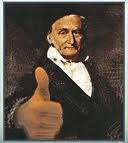
\includegraphics[width=4cm]{gauss}
\caption{Gauss dando legal com largura de 4~cm.}
\label{fig:LeGauss1}
\end{minipage}
\hfill
\begin{minipage}[t]{0.3\linewidth}
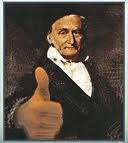
\includegraphics[height=3cm]{gauss}
\caption{Gauss dando legal com altura de 3~cm.}
\label{fig:LeGauss2}
\end{minipage}
\hfill
\begin{minipage}[t]{0.3\linewidth}
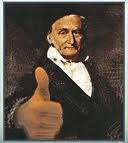
\includegraphics[width=3.3cm,height=1cm]{gauss}
\caption{Gauss?}
\label{fig:LeGauss3}
\end{minipage}
\end{figure}

A Figura~\ref{fig:LeGauss1} foi obtida usando 4~\,cm de largura.
Para tanto usamos \Verb|width=4cm|.
A Figura~\ref{fig:LeGauss2} foi obtida usando 3~\,cm de altura.
Para tanto usamos \Verb|height=3cm|.
Por fim, a Figura~\ref{fig:LeGauss3} foi obtida usando, simultaneamente, 3.3~\,cm 
de largura e 1~\,cm de altura, ou seja, usamos \Verb|width=3.3cm| e \Verb|height=1cm|.

Veja os comandos separada e respectivamente:

\begin{codigo}{Figura com Largura 4\,cm}{\lapis}
\begin{figure}[!htbp]%<--ambiente para figura
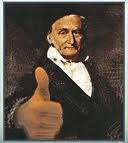
\includegraphics[width=4cm]{gauss}%<--Incluindo a figura
\caption{Gauss dando legal com largura de 4\,cm.}%legenda
\label{fig:LeGauss1}%<--- rótulo
\end{figure}
\end{codigo}

\begin{codigo}{Figura com Altura 3\,cm}{\lapis}
\begin{figure}[!htbp]
  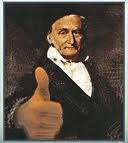
\includegraphics[height=3cm]{gauss}
  \caption{Gauss dando legal com altura de 3\,cm.}
  \label{fig:LeGauss2}
\end{figure}
\end{codigo}

\begin{codigo}{Figura com Largura 3.3\,cm e Altura 1\,cm}{\lapis}
\begin{figure}[!htbp]
  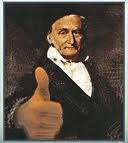
\includegraphics[width=3.3cm,height=1cm]{gauss}
  \caption{Gauss?}
  \label{fig:LeGauss3}
\end{figure}
\end{codigo}

Talvez você esteja se perguntando como colocamos figura ao lado de figura não é 
mesmo?
Mas, veremos isso quando falarmos sobre \texttt{minipage}.

Por hora, vamos analisar como colocar figura em toda margem ou em parte dela.

Ora, para que uma figura ocupe certa proporção da margem disponível à escrita, 
basta usar o comando \verb|width = x\linewidth|.
Onde ``\Verb|x|'' é a proporção (contração) que deseja da margem.\mn{
  Note que $x\in\left(0, 1\right]$.
}
Por exemplo, as Figuras~\ref{fig:amargosa1}~e~\ref{fig:amargosa2}, representam, 
respectivamente, a totalidade da margem em uso (\verb|1\linewidth|) e $30\%$ da 
margem em uso.

\begin{figure}[!htbp] 
\centering 
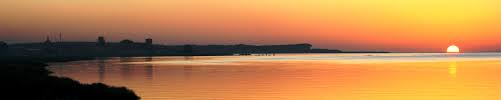
\includegraphics[width=1\linewidth]{por} 
\caption{Foto ocupando toda margem em uso}
\label{fig:amargosa1}
\end{figure}

\begin{figure}[!htbp] 
\centering 
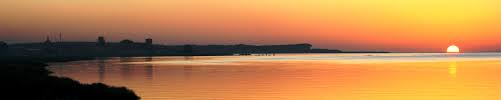
\includegraphics[width=0.3\linewidth]{por}
\caption{Foto ocupando 0.3 da margem em uso}
\label{fig:amargosa2}
\end{figure}

\newpage 

Os respectivos comandos são:

\begin{codigo}{Figuras em diferentes larguras}{\lapis}
\begin{figure}[!htbp] 
  \centering 
  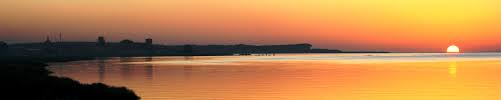
\includegraphics[width=1\linewidth]{por} 
  \caption{Foto ocupando toda margem em uso}
  \label{fig:amargosa1}
\end{figure}

\begin{figure}[!htbp] 
  \centering 
  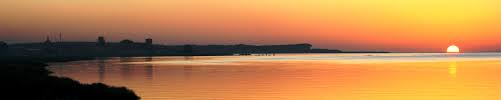
\includegraphics[width=0.3\linewidth]{por}
  \caption{Foto ocupando 0.3 da margem em uso}
  \label{fig:amargosa2}
\end{figure}
\end{codigo}

Caso precise rotacionar uma figura em ``$\alpha$'' graus, use a opção 
``\texttt{angle=$\alpha$}'' como parâmetro.\mn{
  Caso queira citar uma figura específica dentro do texto, o comando é o mesmo 
  usado na citação de tabelas:
  \texttt{\textbackslash \textcolor{azulUFRB}{ref}\{marcação\}}.
}

Veja as Figuras~\ref{fig:avi2} e \ref{fig:avi3} para referência.

\begin{figure}[!htbp]
	\centering
		\begin{minipage}[t]{0.48\linewidth}
			\begin{center}
				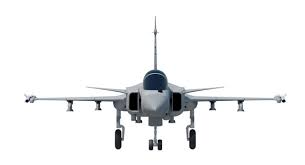
\includegraphics[width=3cm, angle=45]{aviao}
			\end{center}
					\caption{Avião rotacionado em $45^{\circ}$.}
					\label{fig:avi2}
		\end{minipage}
\hfill
		\begin{minipage}[t]{0.48\linewidth}
			\begin{center}
				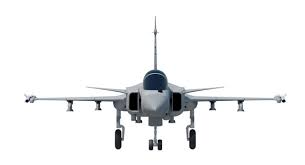
\includegraphics[width=3cm, angle=90]{aviao}
			\end{center}
				\caption{Avião rotacionado em $90^{\circ}$.}
				\label{fig:avi3}
		\end{minipage}
\end{figure}

Os comandos são, respectivamente:

\begin{codigo}{Rotação em $45^{\circ}$}{\lapis}
\begin{figure}[!htbp]
\centering
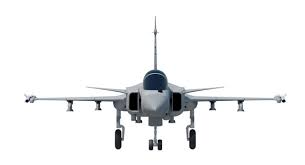
\includegraphics[width=3cm, angle=45]{aviao}
\caption{Avião rotacionado em $45^{\circ}$.}
\label{fig:avi2}
\end{figure}
\end{codigo}

\begin{codigo}{Rotação em $90^{\circ}$}{\lapis}
\begin{figure}[!htbp]
\centering
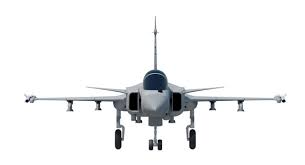
\includegraphics[width=3cm, angle=90]{aviao}
\caption{Avião rotacionado em $90^{\circ}$.}
\label{fig:avi3}
\end{figure}
\end{codigo}

Também é possível inserir uma figura ao longo de uma linha.
Como exemplo, considere o símbolo do cérebro treinando \fbox{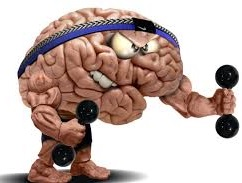
\includegraphics[scale=0.18]{treino}}.

Para tanto, usamos o código:

\begin{codigo}{Figura \textit{inline}}{\lapis}
... treinando \fbox{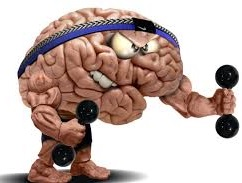
\includegraphics[scale=0.18]{treino}}
\end{codigo}

Note que para deixar o contorno de uma ``caixa'', escrevemos dentro de 
\Verb|\fbox{}|.
Caso não queira o contorno, escreva simplesmente:

\tcboxC{
  \texttt{\textbackslash includegraphics[scale=0.18]\{treino\}}
}

%
  \section{Rodapé e Minipage} %-------------------------------------------------
  \label{sec:pemini}
%
%
  \subsection{Rodapé}
%
Para inserir uma \textit{nota de rodapé} use o comando: \Verb|\footnote{}|.

\begin{tcblisting}{}
\ldots isso completa a demonstração do lema\footnote{Esse resultado vale para 
um caso mais geral, onde $n$ é negativo ou zero.}
\end{tcblisting}

%
  \subsection{Minipage}
%

O ambiente \texttt{minipage}, como o próprio nome sugere, cria uma ``mini página'' 
dentro do texto.
Sua sintaxe, básica, é algo como:

\begin{codigo}{Sintax básica do ambiente \texttt{minipage}}{\lapis}
\begin{minipage}[posição]{comprimento_1}
  <conteúdo da primeira minipage>
\end{minipage}
\hfill
\begin{minipage}[posição]{comprimento_2}
  <conteúdo da segunda minipage>
\end{minipage}
\end{codigo}

Onde \texttt{comprimento\_1} e \texttt{comprimento\_2} especifica a largura de 
cada \textit{minipage}.\mn{ 
  Cuidado para que a soma das larguras das ``minipaginas'' não ultrapasse a largura da página!
}
Eles podem ser substituídos por \texttt{$k$\textbackslash linewidth}, com 
$k\in(0,\,1]$; caso você queira uma proporção da largura do \texttt{minipage} 
com a largura da página.
Além disso, em \texttt{posição}, podemos colocar os parâmetros ``\texttt{t}'', 
``\texttt{c}'', ``\texttt{b}'' para alinhar no topo da \texttt{minipage}, no 
centro ou no final desse ambiente.
Certamente você pode trocar o comando \Verb|\hfill| por algum espaçamento que 
achar conveniente.

Para exemplificar, vamos colocar figura ao lado de figura, como as Figuras~\ref{fig:praca} e
a Figura~\ref{fig:bosque}.

\begin{figure}[!htbp]
	\begin{minipage}[b]{0.45\linewidth}
	\centering
	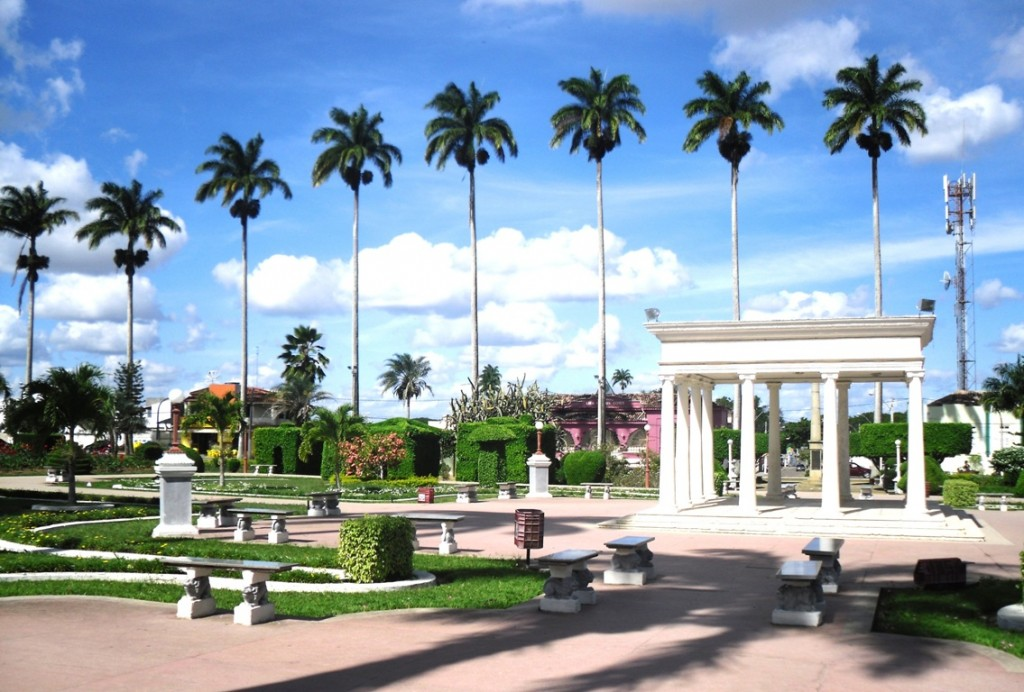
\includegraphics[width=5cm]{praca}
	\caption{Jardim de Amargosa}
	\label{fig:praca}
	\end{minipage}
	\hfill
	\begin{minipage}[b]{0.45\linewidth}
	\centering
	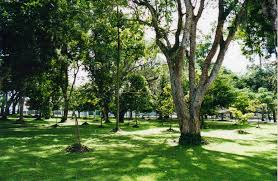
\includegraphics[width=5cm]{bosque}
	\caption{Bosque de Amargosa}
	\label{fig:bosque}
	\end{minipage}
\end{figure}

Perceba nos comandos abaixo, a localização do \textit{minipage}: dentro do 
ambiente \textit{figure}!
Além disso, note onde os comandos de centralização estão localizados também.

Veja os comandos\nota{ 
  Como você faria um cabeçalho básico para sua escola usando combinações de 
  elementos que aprendemos até aqui?
}:

\begin{codigo}{Figura ao lado de figura com \texttt{minipage}}{\lapis}
\begin{figure}[!htbp]
	\begin{minipage}[b]{0.45\linewidth}
	\centering
	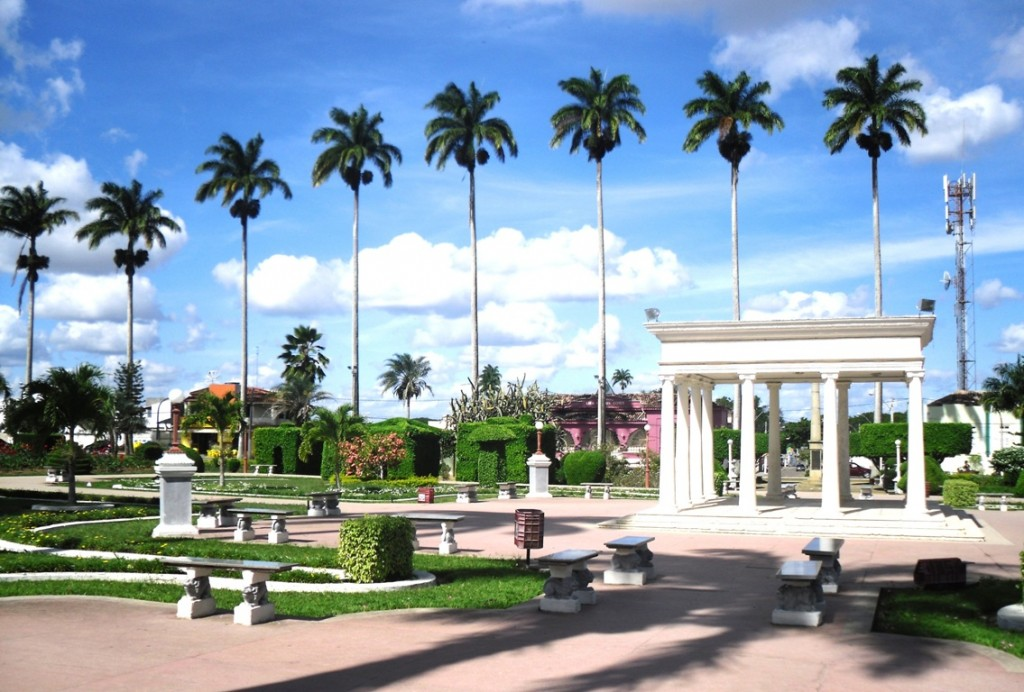
\includegraphics[width=5cm]{praca}
	\caption{Jardim de Amargosa}
	\label{fig:praca}
	\end{minipage}
	\hfill
	\begin{minipage}[b]{0.45\linewidth}
	\centering
	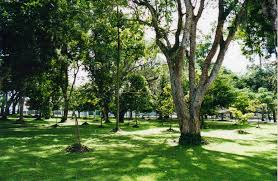
\includegraphics[width=5cm]{bosque}
	\caption{Bosque de Amargosa}
	\label{fig:bosque}
	\end{minipage}
\end{figure}
\end{codigo}

%-------------------------------------------------------------------------------
\newpage